\documentclass[10pt]{article}
\textheight=9.25in \textwidth=7in \topmargin=-.75in
 \oddsidemargin=-0.25in
\evensidemargin=-0.25in
\usepackage{url}  % The bib file uses this
\usepackage{graphicx} %to import pictures
\usepackage{amsmath, amssymb}
\usepackage{theorem, multicol, color}
\usepackage{gfsartemisia-euler}

\setlength{\intextsep}{5mm} \setlength{\textfloatsep}{5mm}
\setlength{\floatsep}{5mm}
\setlength{\parindent}{0em} % new paragraphs are not indented
\setcounter{MaxMatrixCols}{20}
\usepackage{caption}
\captionsetup[figure]{font=small}


%%%%  SHORTCUT COMMANDS  %%%%
\newcommand{\ds}{\displaystyle}
\newcommand{\Z}{\mathbb{Z}}
\newcommand{\arc}{\rightarrow}
\newcommand{\R}{\mathbb{R}}
\newcommand{\N}{\mathbb{N}}
\newcommand{\Q}{\mathbb{Q}}
\renewcommand{\P}{\mathbb{P}}
\newcommand{\blank}{\underline{\hspace{0.33in}}}
\newcommand{\qand}{\quad and \quad}
\renewcommand{\stirling}[2]{\genfrac{\{}{\}}{0pt}{}{#1}{#2}}
\newcommand{\dydx}{\ds \frac{d y}{d x}}
\newcommand{\ddx}{\ds \frac{d}{d x}}
\newcommand{\dvdx}{\ds \frac{d v}{d x}} 
\newcommand{\solution}{\color{blue} Solution: \color{black}}
%%%%  footnote style %%%%

\renewcommand{\thefootnote}{\fnsymbol{footnote}}

\pagestyle{empty}

\begin{document}

\begin{flushright}
Chandler Justice - A02313187
\end{flushright}
\noindent \underline{\hspace{3in}}\\
\textbf{MATH 6400} Quiz \#2\\
\textbf{Due:} January 16, 2026 @ 23:29\\

	\begin{enumerate}
		\item Prove that the infinite series 
		$$S= \sum_{k \geq 1} d_k10^{-k}$$
		is convergent, where $d_k \in \{0,1,2,3,4,5,6,7,8,9\}$. 
		
		Recall the relevance of this: Any real number $x$ is represented by, for all intents and purposes, $N+S$, where $N$ is some integer (and $S$ is an infinite series as above).  
		For example, if $x = 1/3$, then $N = 0$ and $d_k = 3$ for every $k \geq 1$.
		For another, if $x = 4$, then $N = 4$, and $d_k = 0$ for every $k \geq 1$. \\

        \solution If we expand $S$ above, we can see that we get a value of the following shape

        \[0.d_1d_2d_3d_4\cdots\]

        An example of how this could look for some set $d_k \in D$ could be

        \[0.1 + 0.01 + 0.003 + 0.005 + \cdots = 0.1135\cdots\]

 Let

    \[s_n = \sum_{k = 1}^n d_k 10^{-k}\]
    then we can see
\[0 \leq s_n = \sum_{k = 1}^n d_k 10^{-k} \leq \sum_{k = 1}^n 9 \cdot 10^{-k} \leq \sum_{k = 1}^\infty 9 \cdot 10^{-k} = 1.\]

Recall $\sum_{k \geq 1} 9 \cdot 10^{-k}$ is geometric and therefore

\[\sum_{k \geq 1} 9 \cdot 10^{-k} = 9 \cdot \frac{10^{-1}}{1 - 10^{-1}} = 9 \cdot \frac{1/10}{9/10} = 1\]
    
We can also observe it is increasing as $s_{n + 1} - s_n = d_{n+1} 10^{-(n + 1)} \geq 0$

    As $s_n$ is increasing and bounded above by $1$, we conclude that it converges and therefore $S$ also converges. Since we are able to establish the convergence of $S$, we can also confirm $N + S$ is convergent since $N$ is an integer. $\hfill\blacksquare$ 
		
		\item How might the Greeks have convinced themselves that there are incommensurable numbers?  
		In class on 1/16, a proof that there are incommensurable numbers will be presented.  In particular, it will be shown that the diagonal of a square is incommensurable to its sides.  
		The proof will involve modern notation and algebraic moves that the ancients did not have access to.  
		In contrast to the argument mentioned above, the following figure is considered by many to be a possible starting point 
		for how the ancients (in particular, the Greeks) may have faced the fact that there are incommensurable numbers.  
		
		\begin{center}
			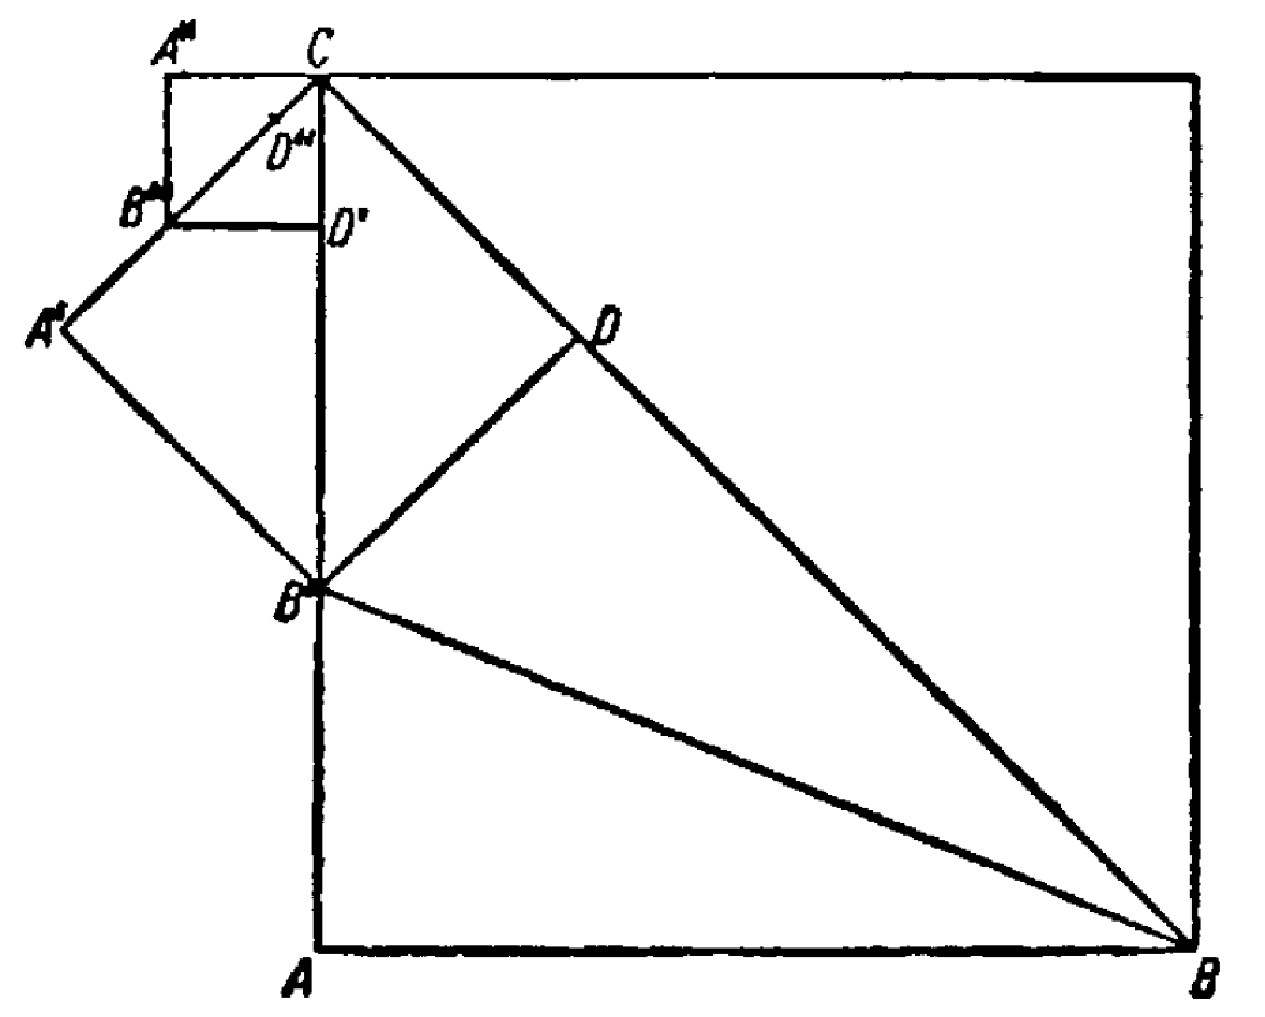
\includegraphics[scale=0.4]{Square_for_incommensurable.pdf}
		\end{center}
		
		Start with the large square with the $3$ corners $A, B,$  and $C$, and diagonal $BC$.  
		Then create $D$ so that $BD$ is the same length as $AB$. 
		Create $B'D$ perpendicular to $BC$ at $D$ intersecting $AC$ at $B'$.
		\emph{Show that $\Delta ABB' \cong \Delta DBB'$}.
		Create the square $A'B'DC$.  
		Create $B'D'$ with the same length as $B'D$.
		Repeat the construction creating the sequence of squares 
		$$A''B''D'C, \;\;\; A'''B'''D''C, \;\;\; A''''B''''D'''C, \;\;\dots $$
		Now, assume $AB$ and $BC$ are commensurable; deduce that $A'B'$ and $B'C$ are commensurable.
		Complete the argument, deriving a contradiction.  Conclude that $AB$ and $BC$ cannot be commensurable.
		
		The conclusion of your proof should involve a fact that (as critics are wont to point out) Euclid did not state.  This fact about (in our terms) a sequence of decreasing positive integers is used in Book VII, Proposition 2. Joyce comments on this unstated assumption in the commentary to Book VII.\\
		
        \solution We start with a square with 3 corners $A,B,C$ which form the sides of a right triangle. We can then see there exists a line between $C$ and $B$ we denote $BC$. Using the line $AB$, measure the line $BC$ and denote this point $D$ such that $AB = BD$. Now, draw a line which in perpendicular to $BC$ towards the line $AC$ whose origin is the point $D$ and terminates on the line $AC$. Denote this point $B'$ and the constructed line $B'D$. We can see that we now have two triangles created with points $ABB'$ and $DBB'$. These triangles are congruent to one another as the lines $BD$ and $AB$ are the same by construction, $BB'$ is a line shared by both triangles and both triangles are right triangles since $ABB'$ is constructed in the corner of the square, and $DBB'$ was constructed with a line perpendicular to the line $BC$. From here, we can mirror the lines $CD$ and $BD$ symmetrically to obtain a new square with points $A', B', C, D$. We can recursively apply the steps taken up to this point to obtain a sequence of squares

		$$A''B''D'C, \;\;\; A'''B'''D''C, \;\;\; A''''B''''D'''C, \;\;\dots $$

Assume $AB$ and $BC$ are commensurable, which is to say there is a unit $u$ such that $AB = mu$ and $BC = nu$ where $n, m \in \Z^+$. Then we can see that must mean $A'B'$ and $B'C$ are also commensurable lines. Since we have constructed an indefinite number of squares using integer lengths, this means this relationship holds for all squares constructed. We can see that as we are obtaining a smaller square at every construction, we will eventually approach a square which cannot be measured by a integers contradicting our construction since there is no infinite decreasing sequence of integers $n, m$. Therefore, $AB$ and $BC$ are not commensurable and there exists incommensurable numbers. $\hfill\blacksquare$
	\end{enumerate}
	


\noindent \underline{\hspace{3in}}\\

\end{document}

